\pdfoutput=1
\documentclass[12pt,a4paper]{article}
\usepackage[utf8]{inputenc}
\usepackage{amsmath}
\usepackage{amsfonts}
\usepackage{amssymb}
\usepackage{amsthm}
\usepackage[margin=0.7in]{geometry}
\usepackage{graphicx}
\usepackage{todonotes}
\usepackage{natbib}
\usepackage{url}
\usepackage[boxruled,vlined,linesnumbered]{algorithm2e}
\usepackage{caption}
\usepackage{subcaption}
\usepackage{lineno}
\usepackage{tcolorbox}
\usepackage{caption}
\usepackage{hyperref}
\usepackage{marginnote}
\AtBeginDocument{\let\textlabel\label}
\hypersetup{colorlinks=true,linkcolor=black,citecolor=black,filecolor=black,urlcolor=black}


\author{Jonathan Rosenblatt \\ Ben Gurion University}

%% OPTIONAL MACRO DEFINITIONS
\renewcommand*{\marginfont}{\scriptsize }

\newcommand{\reals}{\mathbb{R}} % the set of real numbers
\newcommand{\argmin}[2]{\textstyle{\mathop{argmin}_{#1}}\set{#2}} % The argmin operator
\newcommand{\argmax}[2]{\textstyle{\mathop{argmax}_{#1}}\set{#2}} % The argmin operator
\newcommand{\manifold}{\mathcal{M}} % A manifold.
\newcommand{\project}{\hookrightarrow} % The orthogonal projection operator.
\newcommand{\projectMat}{H} % A projection matrix.
\newcommand{\encode}{E} % a linear encoding matrix
\newcommand{\decode}{D} % a linear decoding matrix
\DeclareMathOperator{\Tr}{Tr}
\newcommand{\set}[1]{\{ #1 \}} % A set
\newcommand{\setII}[1]{\left\{ #1 \right\}} % A set
\newcommand{\rv}[1]{\mathbf{#1}} % A random variable
\newcommand{\x}{\rv x} % The random variable x 
\newcommand{\y}{\rv y} % The random variable x 
\newcommand{\U}{\rv u} % The random variable x 
\newcommand{\T}{\rv t} % The random variable x 
\newcommand{\X}{\rv X} % The random variable x 
\newcommand{\Y}{\rv Y} % The random variable y
\newcommand{\expect}[1]{\mathbf{E}\left[ #1 \right]} % The expectation operator
\newcommand{\expectg}[2]{\mathbf{E}_{\rv{#1}}\left[ \rv{#2} \right]} % An expectation w.r.t. a particular random variable.
\newcommand{\expectn}[1]{\mathbb{E}\left[#1\right]} % The empirical expectation
\newcommand{\cov}[1]{\mathbf{Cov} \left[ #1 \right]} % The expectation operator
\newcommand{\var}[1]{\mathop{Var} \left[ #1 \right]} % The expectation operator
\newcommand{\covn}[1]{\mathbb{Cov} \left[ #1 \right]} % The expectation operator
\newcommand{\gauss}[1]{\mathcal{N}\left(#1\right)} % The gaussian distribution
\newcommand{\cdf}[2]{F_{#1} (#2)} % The CDF function
\newcommand{\survive}[2]{S_{#1} (#2)} % The survival function
\newcommand{\hazard}[2]{h_{#1} (#2)} % The survival function
\newcommand{\cuhazard}[2]{H_{#1} (#2)} % The survival function
\newcommand{\cdfn}[2]{\mathbb{F}_{#1}(#2)} % The empirical CDF function
\newcommand{\icdf}[2]{F_\rv{#1}^{-1} (#2)} % The invecrse CDF function
\newcommand{\icdfn}[2]{\mathbb{F}^{-1}_{#1}(#2)} % The inverse empirical CDF function
\newcommand{\pdf}[2]{p_{#1} (#2)} % The CDF function
\newcommand{\prob}[1]{P\left( #1 \right)} % the probability of an event
\newcommand{\dist}{P} % The proabaiblity distribution
\newcommand{\density}{p}
\newcommand{\entropy}{H} % entropy
\newcommand{\mutual}[2]{I\left(#1;#2\right)} % mutual information
\newcommand{\norm}[1]{\Vert #1 \Vert} % The norm operator
\newcommand{\normII}[1]{\norm{#1}_2} % The norm operator
\newcommand{\normI}[1]{\norm{#1}_1} % The norm operator
\newcommand{\normF}[1]{\norm{#1}_{Frob}} % The Frobenius matrix norm
\newcommand{\ones}{\textbf{1}} % Vector of ones.
\newcommand{\lik}{\mathcal{L}} % The likelihood function
\newcommand{\loglik}{L} % The log likelihood function
\newcommand{\loss}{l} % A loss function
\newcommand{\lossII}{\prescript{}{2}{l}} % A loss function
\newcommand{\risk}{R} % The risk function
\newcommand{\riskn}{\mathbb{R}} % The empirical risk
\newcommand{\riskII}{\prescript{}{2}{R}} % The empirical risk
\newcommand{\risknII}{\prescript{}{2}{\mathbb{R}} } % The empirical risk
\newcommand{\noisen}{\mathbb{G}} % The empirical noise process
\newcommand{\deriv}[2]{\frac{\partial #1}{\partial #2}} % A derivative
\newcommand{\hyp}{f} % A hypothesis
\newcommand{\hypclass}{\mathcal{F}} % A hypothesis class
\newcommand{\hilbert}{\mathcal{H}}
\newcommand{\rkhs}{\hilbert_\kernel} % A hypothesis class
\newcommand{\normrkhs}[1]{\norm{#1}_{\rkhs}} % the RKHS function norm
\newcommand{\rank}{q} % A subspace rank.
\newcommand{\dimy}{K} % The dimension of the output.
\newcommand{\latent}{\rv{s}} % latent variables matrix
\newcommand{\latentn}{S} % latent variables matrix
\newcommand{\loadings}{A} % factor loadings matrix
\newcommand{\rotation}{R}  % rotation matrix
\newcommand{\similaritys}{\mathfrak{S}} % a similarity graph
\newcommand{\similarity}{s} % A similarity measure.
\newcommand{\dissimilarity}{d} % A dissimilarity measure.
\newcommand{\dissimilaritys}{\mathfrak{D}} % a dissimilarity graph
\newcommand{\scalar}[2]{\left< #1,#2 \right>} % a scalar product
\newcommand{\aka}{{a.k.a.\ }}
\newcommand{\Aka}{{A.k.a.\ }}









\theoremstyle{plain}
\newtheorem{theorem}{Theorem}[section]
\newtheorem*{theorem*}{Theorem}
\newtheorem{lemma}{Lemma}[section]
\newtheorem*{lemma*}{Lemma}
\newtheorem{prop}{Proposition}[section]
\newtheorem{cor}{Corollary}[section]


\theoremstyle{definition}
\newtheorem{definition}{Definition}
\newtheorem{remark}{Remark}
%\newtheorem{think}{Gedankenexperiment}
%\newtheorem*{think}{Think about it \faLightbulbO}

\newtheorem{example}{Example}

\newenvironment{think}
	{
		\bigskip
		\begin{tcolorbox}
		\paragraph{Think about it.}
	}{
		\end{tcolorbox}
}

\newenvironment{extra}
{
	\bigskip
	\begin{tcolorbox}
		\paragraph{Extra Information.}
	}{
	\end{tcolorbox}
}



% Custom commands

\newcommand{\naive}{na\"{\i}ve }
\newcommand{\Naive}{Na\"{\i}ve }
\newcommand{\andor}{and\textbackslash or }
\newcommand{\erdos}{Erd\H{o}s }
\newcommand{\renyi}{R\`enyi }


\title{Dimensionality Reduction}


\begin{document}

\maketitle

\begin{example}[BMI]
	\label{ex:bmi}
	Consider the heights and weights of a sample of individuals. 
	The data may seemingly reside in $2$ dimensions but given the height, we have a pretty good guess of a person's weight, and vice versa. 
	We can thus state that heights and weights are not really two dimensional, but roughly lay on a $1$ dimensional subspace of $\reals^2$. 
\end{example}


\begin{example}[IQ]
	\label{ex:iq}
	Consider the correctness of the answers to a questionnaire with $p$ questions. 
	The data may seemingly reside in a $p$ dimensional space, but assuming there is such a thing as ``skill'', then given the correctness of a person's reply to a subset of questions, we have a good idea how he scores on the rest. 
	Put differently, we don't really need a $200$ question questionnaire-- $100$ is more than enough.
	If skill is indeed a one dimensional quality, then the questionnaire data should organize around a single line in the $p$ dimensional cube. 
\end{example}


\begin{example}[Blind signal separation]
	\label{ex:blind-signal}
	Consider $n$ microphones recording an individual. 
	The digitized recording consists of $p$ samples. 
	Are the recordings really a shapeless cloud of $n$ points in $\reals^p$?
	Since they all record the same sound, one would expect them to arrange around a single 
\end{example}
		
	


\section{General Terminology}

\begin{tcolorbox}
\begin{description}
	\item[Data] \Aka \emph{sample}, \emph{observations}, depending on your community. 
	Will typically consist of $n$, $p$ dimensional vectors.
	We typically denote the data as an $n\times p$ matrix $X$. 
	
	\item[Manifold] A space which is regular enough so that it is \emph{locally} has all the properties of a linear space. 
	We will denote an arbitrary manifold by $\manifold$.
	
	
	\item[Embedding] Informally speaking: a ``shape preserving'' mapping of a space into another. 
	
	\item[Linear Embedding] An embedding done via a linear operation (thus representable by a matrix). 
	
	\item[Generative Model] Known to statisticians as the \emph{sampling distribution}. 
	The assumed stochastic process that generated the observed data. 
	
\end{description}
\end{tcolorbox}





\section{Principal Component Analysis}
\label{sec:pca}

\emph{Principal Component Analysis} (PCA) is such a basic technique, it has been rediscovered and renamed independently in many fields. 
It can be found under the names of 
\emph{
	Discrete Karhunen–Loève Transform; 
	Hotteling Transform; 
	Proper Orthogonal Decomposition (POD); 
	Eckart–Young Theorem; 
	Schmidt–Mirsky Theorem;  
	Empirical Orthogonal Functions; 
	Empirical Eigenfunction Decomposition;  
	Empirical Component Analysis;  
	Quasi-Harmonic Modes;  
	Spectral Decomposition;  
	Empirical Modal Analysis}, 
and possibly more\footnote{\url{http://en.wikipedia.org/wiki/Principal_component_analysis} }.
The many names are quite interesting as they offer an insight into the different problems that led to PCA's (re)discovery.


Return to the BMI problem in Exampl~\ref{ex:bmi}.
Assume you now wish to give each individual a ``size score'', that is a \textbf{linear} combination of height and weight: PCA does just that. 
It returns the linear combination that has the largest variability, i.e., the combination which best distinguishes between individuals. 

The variance maximizing motivation above was the one that guided Hotelling \citet{hotelling1933analysis}.
But $30$ years before him, \citet{pearson1901liii} derived the same procedure with a different motivation in mind. 
Pearson was also trying to give each individual a score. 
He did not care about variance maximization, however. 
He simply wanted a small set of coordinates in some (linear) space that approximates the original data well. 
As it turns out, the best linear-space approximation of $X$ is also the variance maximizing one. 
More precisely: the \emph{sequence} of $1,\dots,p$ dimensional linear spaces that best approximate $X$, is exactly the sequence of $1,\dots,p$ dimensional scores, that best separate between the $n$ samples. 
Pearson and Hotelling (among others) thus arrived to the exact same solution, with different motivations. 





\subsubsection{Scree Plot}
\label{sec:scree_plot}





\subsubsection{Bi Plot}
\label{sec:bi_plot}
The \emph{Bi-Plot} shows the two first scores of the original data points.
These scores are known as the \emph{Principal Componets} (PCs). \marginnote{Principal Components}
The contribution of each original variable to each PC, is called the \emph{Loadings}.
The plot also shows the contribution of each of the original variables to each of the scores. 
See example in Figure~\ref{fig:usaarrests}.


\begin{figure}[ht]
	\centering
	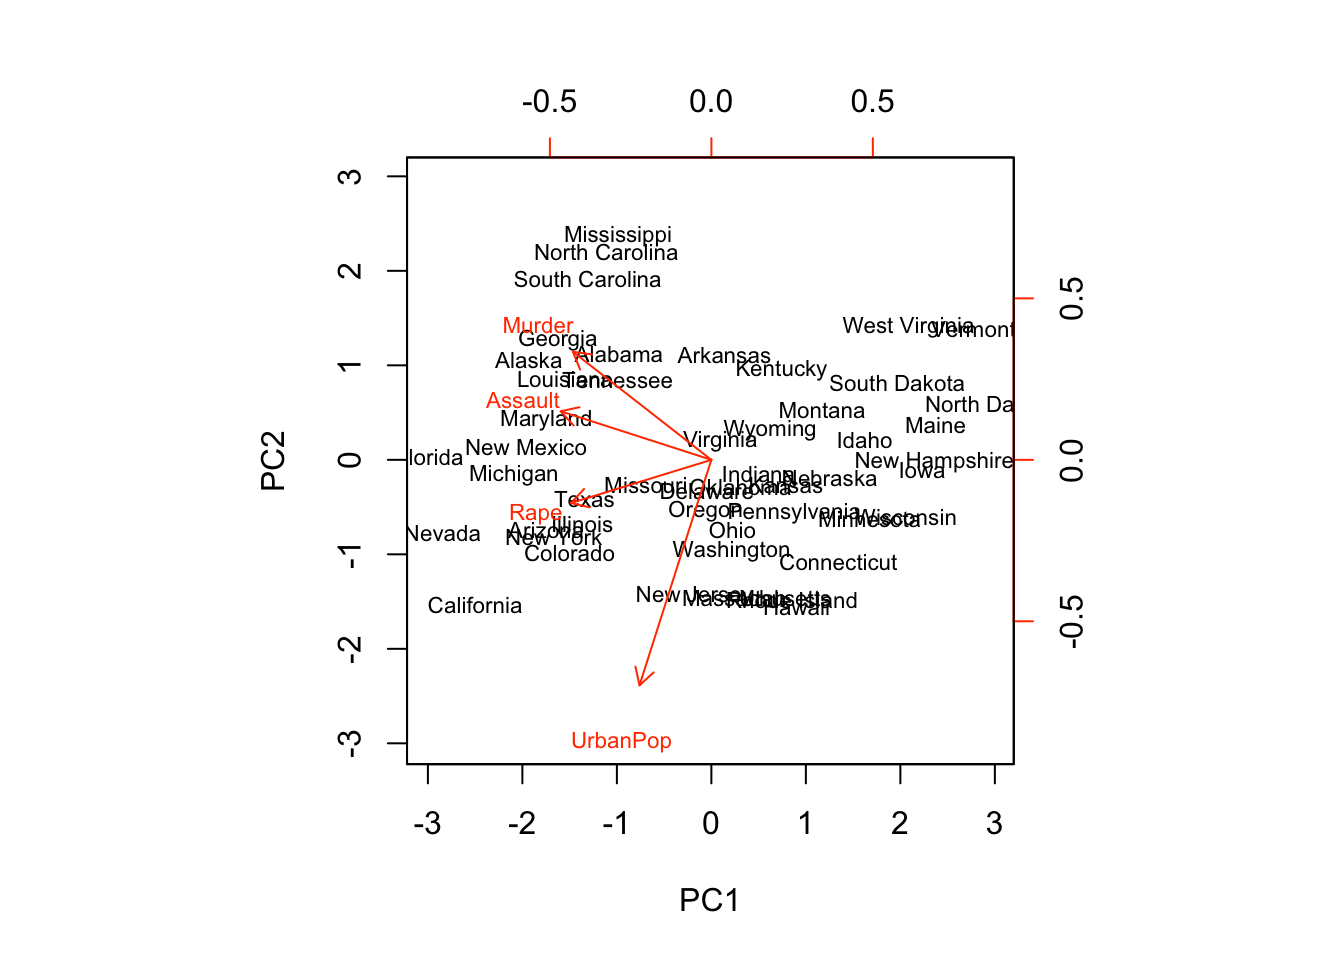
\includegraphics[width=0.7\linewidth]{USAarrests}
	\caption{\textbf{BiPlot}.
		Arrest type data for USA states. 
		Data includes urban population size, number of rape related arrests, assault related, and murder related ($p=4$). 
		Each city is presented against its two first PCs. 
		Arrows encode the loadings. 
		They show that PC1 encodes a general crime level, as it is the average of all type of crimes. 
		PC2 measures the level of urbanization, as it is dominated by the UrbanPopulation variable. 		
		\\ Source: \url{https://goo.gl/85qtKv}}
	\label{fig:usaarrests}
\end{figure}






\subsubsection{Mathematics of PCA}
\label{sec:pca_mathematics}
We now present the derivation of PCA from the two different motivations.


\begin{proof}
	The sketch of the proof is the following:
	We will first show that the weight vector that maximizes the variance is the eigenvector that corresponds to the first principal component.
	We will do so for the \emph{population} covariance, $\Sigma$, and wrap up by plugging its empirical counterpart, $X'X$ (assuming a centered $X$). 
		
	Starting with the first principal component.
	For a random $p$-vector, $\x$ denote $\Sigma:=\cov{\x}$, so that for a fixed $p$-vector $v$: $\cov{v'\x}=v' \Sigma v$.
	Finding a linear combination of $\x$ that best separates individuals, means maximizing $\cov{v'x}$
	w.r.t. to $v$.
	Clearly, $\cov{v'x}$ may explode if any $v$ is allowed. 
	It is most convenient, mathematically, to constrain the $l_2$ norm: $\normII{v}^2=1$.
	Maximizing under a constraint, using Lagrange-Multipliers: 
	\begin{align}
	\argmax{v}{v \Sigma v' - \lambda (\normII{v}^2-1)}.
	\end{align}
	Differentiating w.r.t $v$ and equating zero: 
	\begin{align}
	(\Sigma- \lambda I) v = 0
	\end{align}
	So the $P$ solutions for $v$ are the eigen-vectors of $\Sigma$. Which of them to pick? 
	To find a \emph{global} maximum we return to the original problem, as plug our result:
	\begin{align}
	\label{eq:pca_maximal_variance}
	\argmax{v:\normII{v}^2=1}{v \Sigma v' }=\argmax{\lambda}{v \lambda v' }
	\end{align}
	so that the global maximum is obtained with the largest eigen-value $\lambda$.
	
	Readers familiar with matrix norms will recognize that this is simply the derivation of the operator norm of $\Sigma$.
	
	The second principal component can be found by solving the same problem, with the additional constraint of $v_2$ orthogonal to $v_1$.
	
	The last missing ingredient is that instead of the true covariance between the features, $\Sigma$, we use the (scaled) empirical covariance $X'X$.
\end{proof}



\paragraph{The Linear-Space Embedding View}
We now seek to find a sequence of $p$ approximations to $X$ that lay in $1,\dots,p$ dimensional linear subspaces, with respect to a least squares loss. For simplicity of exposition, we will assume that $X$ has been mean centred. 
The $\rank$'th problem to solve is thus
\begin{align}
\label{eq:pca_erm}
\argmin{\hyp_\rank}{\normF{X-\hyp_\rank(X)}}.
\end{align}
Since $\hyp_rank$ is a map from $\reals^p$ to some rank-$\rank$ linear subspace, it must have the form $\hyp_\rank(X)=\projectMat_\rank X$ where $\projectMat_\rank$ is a $n \times n$ matrix of rank $\rank$.
Since Eq.(\ref{eq:pca_erm}) minimizes sums of (squared) Euclidean distances, $\projectMat_\rank$ has to be an orthogonal projection, thus symmetric. As such it can decomposed into an outer product $\projectMat_\rank=V_\rank V'_\rank$ where $V_\rank$ is full rank $n \times \rank$ matrix \citep[Eq.(5.13.4)]{meyer_matrix_2001}.
Under the $\rank$-space constraint, and squared error, Eq.(\ref{eq:pca_erm}) collapses to 
\begin{align}
\label{eq:pca_erm2}
\argmin{V_\rank}{\normF{X-V_\rank V'_\rank(X)}}.
\end{align}
Using some algebraic identities \cite[Eq.(23.3)]{shalev-shwartz_understanding_2014} Eq.(\ref{eq:pca_erm2}) is equivalent to 
\begin{align}
\label{eq:pca_erm3}
\argmax{V_\rank}{\Tr(V'_\rank XX' V_\rank)}.		
\end{align}
At this point we should note that the linear-space embedding problem has collapsed to the variance maximization problem! 
If you do not see this, just set $\rank=1$ and compare to Eq.(\ref{eq:pca_maximal_variance}), recalling that $X'X$ estimates the features' covariance $\Sigma$.








\subsubsection{Intuition}
\label{sec:pca_intuition}

Notice we have currently offered two motivations for PCA: 
(i) Find linear combinations that best distinguish between observations, i.e., maximize variance. 
(ii) Find the linear subspace the bets approximates the data.
The reason these two problems are equivalent, is due to the use of the squares error.
Informally speaking, the data has some total variance. 
This variance can be decomposed into the part captured in $\manifold$, and the part not captured\footnote{Analogous to $SST=SSR+SSE$ in linear regression.}. 
Since the variance in the data consists of sums of squares, minimizing the distance from $X$ to $\manifold$, is the same as maximizing the variance of $X \project \manifold$, since their sum is fixed.





\subsubsection{PCA as a Graph Method}
\label{remark:pca_as_graph}
Starting from the maximal variance motivation, it is perhaps not surprising that PCA depends only on the similarities between features, as measured by their empirical covariance. The linearity of the target manifold was there by assumption. 

Following the linear-space embedding motivation, it is was surprising that the solutions depend only on the empirical covariances. This fact can be attributed to the use of squared error loss, which implied we were trying to decompose the total variance into the part in $\manifold_\rank$ and the orthogonal part.

From both motivations we see that the values of $X$ are of no importance given $X'X$, which can be informally thought of as a sufficient statistic\footnote{It is not a proper sufficient statistic as no generative model has been assumed.}.  

In-turn, $X'X$ depends only on the empirical covariances between \emph{individuals} ($\similaritys=XX'$), or on the Euclidean distances between individuals ($\dissimilaritys=(\norm{x_i-x_j})$).

The building blocks of all these graph-based dimensionality reduction methods are:
\begin{enumerate}
	\item Compute some similarity graph $\similaritys$ (or dissimilarity graph $\dissimilaritys$) from the raw features.
	\item Call upon graph embedding theory to map the data points into the target manifold $\manifold$.
\end{enumerate}
The fact that the linear-space embedding of the data depends only some similarity graph has laid a bridge between feature embedding, such as PCA, and \emph{graph embedding} methods such as MDS (\S\ref{sec:mds}).
Moreover, it has opened the door for replacing the covariance similarity, with many other similarity measures. 
Classic MDS (\S\ref{sec:mds}) is simply PCA when starting from $\similaritys$, thus viewed as a graph embedding problem.
kPCA (\S\ref{sec:kpca}) plugs kernel similarities (\S\ref{apx:rkhs}) instead of covariance similarities. 
Isomap (\S\ref{sec:isomap}), LocalMDS (\S\ref{sec:localMDS}), and LLE (\S\ref{sec:lle}) follow a similar motivation using \emph{local} measures of similarity.
Spectral Clustering (\S\ref{sec:spectral_clustering}) does some linear-space embedding \`a-la PCA, then wrapping up with a clustering algorithm in $\manifold$ \`a-la K-means. 



We now prove that the PCA solution can be cast in terms of the covariance between individuals ($\similaritys=XX'$) or the Euclidean distances ($\dissimilaritys=\norm{x_i-x_j}$).
In particular, we show that all the information on the location (mean) of $X$, needed for the PCA reconstruction, is actually encoded in $\similaritys$ (or $\dissimilaritys$).

The following exposition takes from \cite[Section 18.5.2]{hastie_elements_2003}


\paragraph{PCA with the Covariance Similarity Graph}
To begin, we need to cast the solution to the PCA problem in Eq.(\ref{eq:pca_erm3}) using the Singular Value Decomposition (SVD).\marginnote{SVD}

\begin{definition}[SVD]
	Any $n \times p$ matrix $X$, can be decomposed into $X=UDV'$ where 
	$U$ is an $n \times p$ orthogonal matrix ($U'U=I_p$); 
	$D$ is a $p \times p$ diagonal matrix with diagonal elements $d_1 \geq d_2 \geq \dots \geq d_p$;
	$V$ is a $p \times p$ orthogonal matrix ($V'V=I_p$).
\end{definition}

For mean centered $X$, the series of embeddings $\hyp_\rank(X)$ for $\rank=1,\dots,\pagebreak$ resulting from Eq.(\ref{eq:pca_erm3}) is given by $\hyp_\rank(X)=U_\rank D_\rank$, where $U_\rank$ $D_\rank$ are the $\rank$ leading columns of $U$ and $D$ respectively. $UD$ is thus the sequence of all solutions.

Now denoting $\similaritys=XX'$ and calling SVD: $\similaritys=U D^2 U'$. 
We thus see that by decomposing $\similaritys$ we can recover $U$, $D$, and thus $\hyp_\rank(X)$.

If $X$ is not mean centred, the relation still holds, but we skip the presentation.


\paragraph{PCA with the Euclidean Distance Dissimilarity Graph}
Can we convert Euclidean distances to empirical covariances? Yes!

Denote the matrix of distances of a non-centred $X$: $\dissimilaritys^2=(\norm{x_i-x_j}^2)$.
\begin{align}
\dissimilaritys^2_{i,j} =& \norm{x_i-x_j}^2 \\
=& \normII{x_i-\bar{x}}+\normII{x_j-\bar{x}}-2 \scalar{x_i-\bar{x}}{x_j-\bar{x}} \\
=& \normII{x_i-\bar{x}}+\normII{x_j-\bar{x}}-2 \similaritys_{i,j}
\end{align}
where $\similaritys_{i,j}$ is the empirical covariance between individual $i$ and $j$.
We thus have 
\begin{align}
\similaritys= - (I-M) \frac{\dissimilaritys^2}{2} (I-M)
\end{align}
where $M$ is the centring matrix: $M:= \frac{1}{n} \ones \ones'$, and $\ones$ an $n$ vector of $1$'s.







\section{FA}




\section{ICA}






\newpage
\bibliographystyle{abbrvnat}
\bibliography{dim_reduce.bib}



\end{document}
